\section{Accessibilità}
\subsection{Separazione tra struttura, presentazione e comportamento}
Per migliorare l'accesso al sito a qualsiasi categoria di utenti è stata mantenuta la separazione tra struttura, presentazione e comportamento. \\
La prima è stata sviluppata tramite documenti HTML5. Questi richiamano i fogli di stile esterni CSS, che implementano la presentazione, e gli script esterni di JavaScript che ne determinano il comportamento.
\subsection{Tag meta}
Per ogni pagina web sono stati inseriti i seguenti tag meta:
\begin{itemize}
	\item \textbf{title}: titolo;
	\item \textbf{description}: descrizione sintetica;
	\item \textbf{keywords}: lista di parole chiave che permette di specificare gli argomenti trattati;
	\item \textbf{author}: indica gli autori della pagina;
	\item \textbf{viewport}: utilizzato per "comunicare" al browser come adattare il sito per dispositivi con diverse misure.
\end{itemize}


\subsection{Percepibilità}
La percepibilità consiste in: 
	\begin{itemize}
		\item fornire alternative testuali per qualsiasi contenuto non testuale, in modo che questo possa essere trasformato in altre forme fruibili secondo le necessità degli utenti;
		\item rendere più semplice agli utenti la visione dei contenuti.
	\end{itemize}
	In particolare il gruppo ha seguito queste regole:
	\begin{itemize}
		\item attributo \textit{alt} con un appropriato testo sostitutivo a tutte le immagini;
		\item non sono state utilizzate immagini per riportare il testo, rendendo il contenuto informativo accessibile anche agli utenti che utilizzano gli screen reader;
		\item attributo \textit{scope= "col"} per specificare la cella header di una colonna, o gruppo di colonne in una tabella(sempre rivolto agli utenti che utilizzano gli screen reader);
		\item un tag \textit{label} che descrive la finalità di ogni textfield di ogni form;
		\item un tag \textit{legend} per tutti i fieldset, utile a descriverne il contenuto.
	\end{itemize}
\subsubsection{Colori}
Per rendere il più semplice possibile agli utenti la visione dei contenuti è stato adottato un appropriato schema di colori, il quale garantisce un certo contrasto cromatico.
	In particolare, miriamo a dare meno disagi possibili agli utenti affetti da particolari patologie agli occhi, quali deuteranopia, protanopia e tritanopia. \\
	Gli screenshot qui sotto sono una simulazione di come un utente appartenente a questa categoria vede il nostro sito.\\
	\begin{figure}
	\centering
		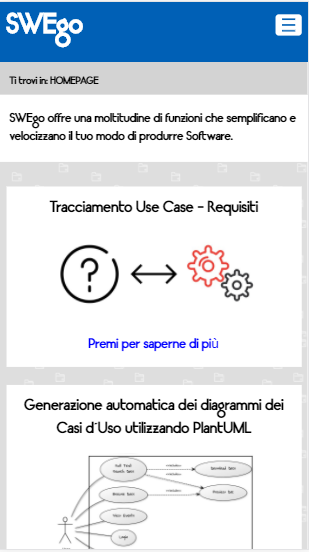
\includegraphics[scale=1]{img/normale_mobile.jpeg}\\[1cm] \caption{Pagina mobile di login vista da un utente normale.}
	\end{figure}
	\begin{figure}
	\centering
		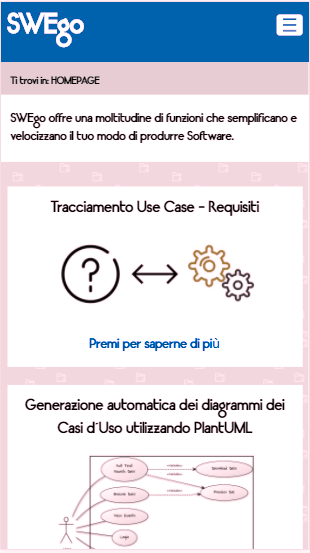
\includegraphics[scale=1]{img/deuteranopia_mobile.png}\\[1cm] \caption{Pagina mobile di login vista da un utente affetto da deuteranopia}
	\end{figure}
	\begin{figure}
	\centering
		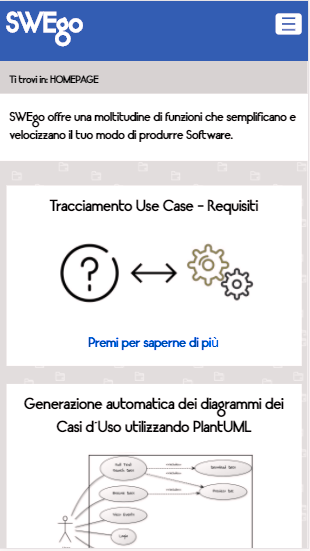
\includegraphics[scale=1]{img/protanopia_mobile.png}\\[1cm] \caption{Pagina mobile di login vista da un utente affetto da protanopia}
	\end{figure}
	\begin{figure}
	\centering
		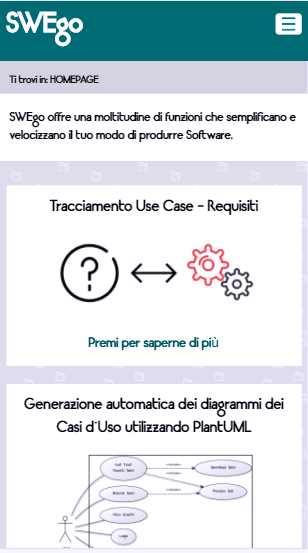
\includegraphics[scale=1]{img/tritanopia_mobile.png}\\[1cm] \caption{Pagina mobile di login vista da un utente affetto da tritanopia}
	\end{figure}
\subsection{Usabilità}
Al fine di migliorare l'esperienza d'uso degli utenti sono state inserite le seguenti facilitazioni:
\begin{itemize}
	\item \textbf{tabindex}: non è stato ridefinito il comportamento del pulsante tab tramite l'attributo tabindex, in quanto il gruppo ritiene quello di default agevole per la navigazione;
	\item \textbf{link per spostarsi al contenuto}: prima della barra di navigazione è stato inserito un link nascosto per saltarla, permettendo agli utenti che utilizzano uno screen reader di passare direttamente al contenuto;
	\item 
\end{itemize}
Inoltre per rendere ben navigabile il sito si è fatto uso di:
\begin{itemize}
	\item breadcrumb, il quale permette di capire in che pagina ci si trova;
	\item mappa del sito;
\end{itemize}
\subsection{Comprensibilità}
Le informazioni del sito devono risultare comprensibili per gli utenti. A tal scopo si è fatto utilizzo di:
	\begin{itemize}
		\item \textit{xml:lang=en} per specificare che alcune parole sono inglesi;
		\item menù quasi uguali per tutte le pagine, rendendo la voce di menù della pagina attuale non cliccabile;
		\item apposite label e istruzioni che aiutano l'utente a inserire dati corretti;
		\item un gruppo di \textit{checkbox} al posto di \textit{<select multiple>}, in quanto risulta molto più comprensibile e di più facile utilizzo.
	\end{itemize}
\subsection{Robustezza}